% VDE Template for EUSAR Papers
% Provided by Barbara Lang und Siegmar Lampe
% University of Bremen, January 2002
% English version by Jens Fischer
% German Aerospace Center (DLR), December 2005
% Additional modifications by Matthias Wei{\ss}
% FGAN, January 2009

%-----------------------------------------------------------------------------
% Type of publication
\documentclass[a4paper,10pt]{article}
%-----------------------------------------------------------------------------
% Other packets: Most packets may be downloaded from www.dante.de and
% "tcilatex.tex" can be found at (December 2005):
% http://www.mackichan.com/techtalk/v30/UsingFloat.htm
% Not all packets are necessarily needed:
\usepackage[T1]{fontenc}
\usepackage[latin1]{inputenc}
%\usepackage{ngerman} % in german language if required
\usepackage[nooneline,bf]{caption} % Figure descriptions from left margin
\usepackage{times}
\usepackage{multicol}
\usepackage{amsmath}
\usepackage{amssymb}
\usepackage{graphicx}
\usepackage{epsfig}
\input{tcilatex}
%-----------------------------------------------------------------------------
% Page Setup
\textheight24cm \textwidth17cm \columnsep6mm
\oddsidemargin-5mm                 % depending on print drivers!
\evensidemargin-5mm                % required margin size: 2cm
\headheight0cm \headsep0cm \topmargin0cm \parindent0cm
\pagestyle{empty}                  % delete footer and header
%----------------------------------------------------------------------------
% Environment definitions
\newenvironment*{mytitle}{\begin{LARGE}\bf}{\end{LARGE}\\}%
\newenvironment*{mysubtitle}{\bf}{\\[1.5ex]}%
\newenvironment*{myabstract}{\begin{Large}\bf}{\end{Large}\\[2.5ex]}%
%-----------------------------------------------------------------------------
% Using Pictures and tables:
% - Instead "table" write "tablehere" without parameters
% - Instead "figure" write "figurehere " without parameters
% - Please insert a blank line before and after \begin{figuerhere} ... \end{figurehere}
%
% CAUTION:   The first reference to a figure/table in the text should be formatted fat.
%
\makeatletter
\newenvironment{tablehere}{\def\@captype{table}}{}
\newenvironment{figurehere}{\def\@captype{figure}\vspace{2ex}}{\vspace{2ex}}
\makeatother



%%%%%%%%%%%%%%%%%%%%%%%%%%%%%%%%%%%%%%%%%%%%%%%%%%%%%%%%%%%%%%%%%%%%%%%%%%%%%%
\begin{document}

% Please use capital letters in the beginning of important words as for example
\begin{mytitle}A survey on resource management policies for NUMA architectures\end{mytitle}
%
% Please do not insert a line here
%
\\
Ferrini Francesco\\
Matr. 755508, (goffredoam84@gmail.com)\\
\hspace{10ex}
Gallo Francesco\\
Matr. 755748, (loshura@hotmail.it)\\
\begin{flushright}
\emph{Report for the master course of Embedded Systems}\\
\emph{Reviser: PhD. Patrick Bellasi (bellasi@elet.polimi.it)}
\end{flushright}

Received: April, 01 2011\\
\hspace{10ex}

\begin{myabstract} Abstract \end{myabstract}
abstract

\vspace{4ex}	% Please do not remove or reduce this space here.
\begin{multicols}{2}

%%%%%%%%%%%%%%%%%%%%%%%%%%%%%%%%%%%%%%%%%%%%%%%%%%%%%%%%%%%%%%%%%%%%%%%%%%%%%
\section{Introduction}

Numa (Non-Uniform Access Memory) refers to a computer memory design choice used in multiprocessing, where the memory access time depends on the memory location relative to a processor; in fact NUMA means that it will take longer to access some regions of memory than others.

\begin{figurehere}
 \centering
 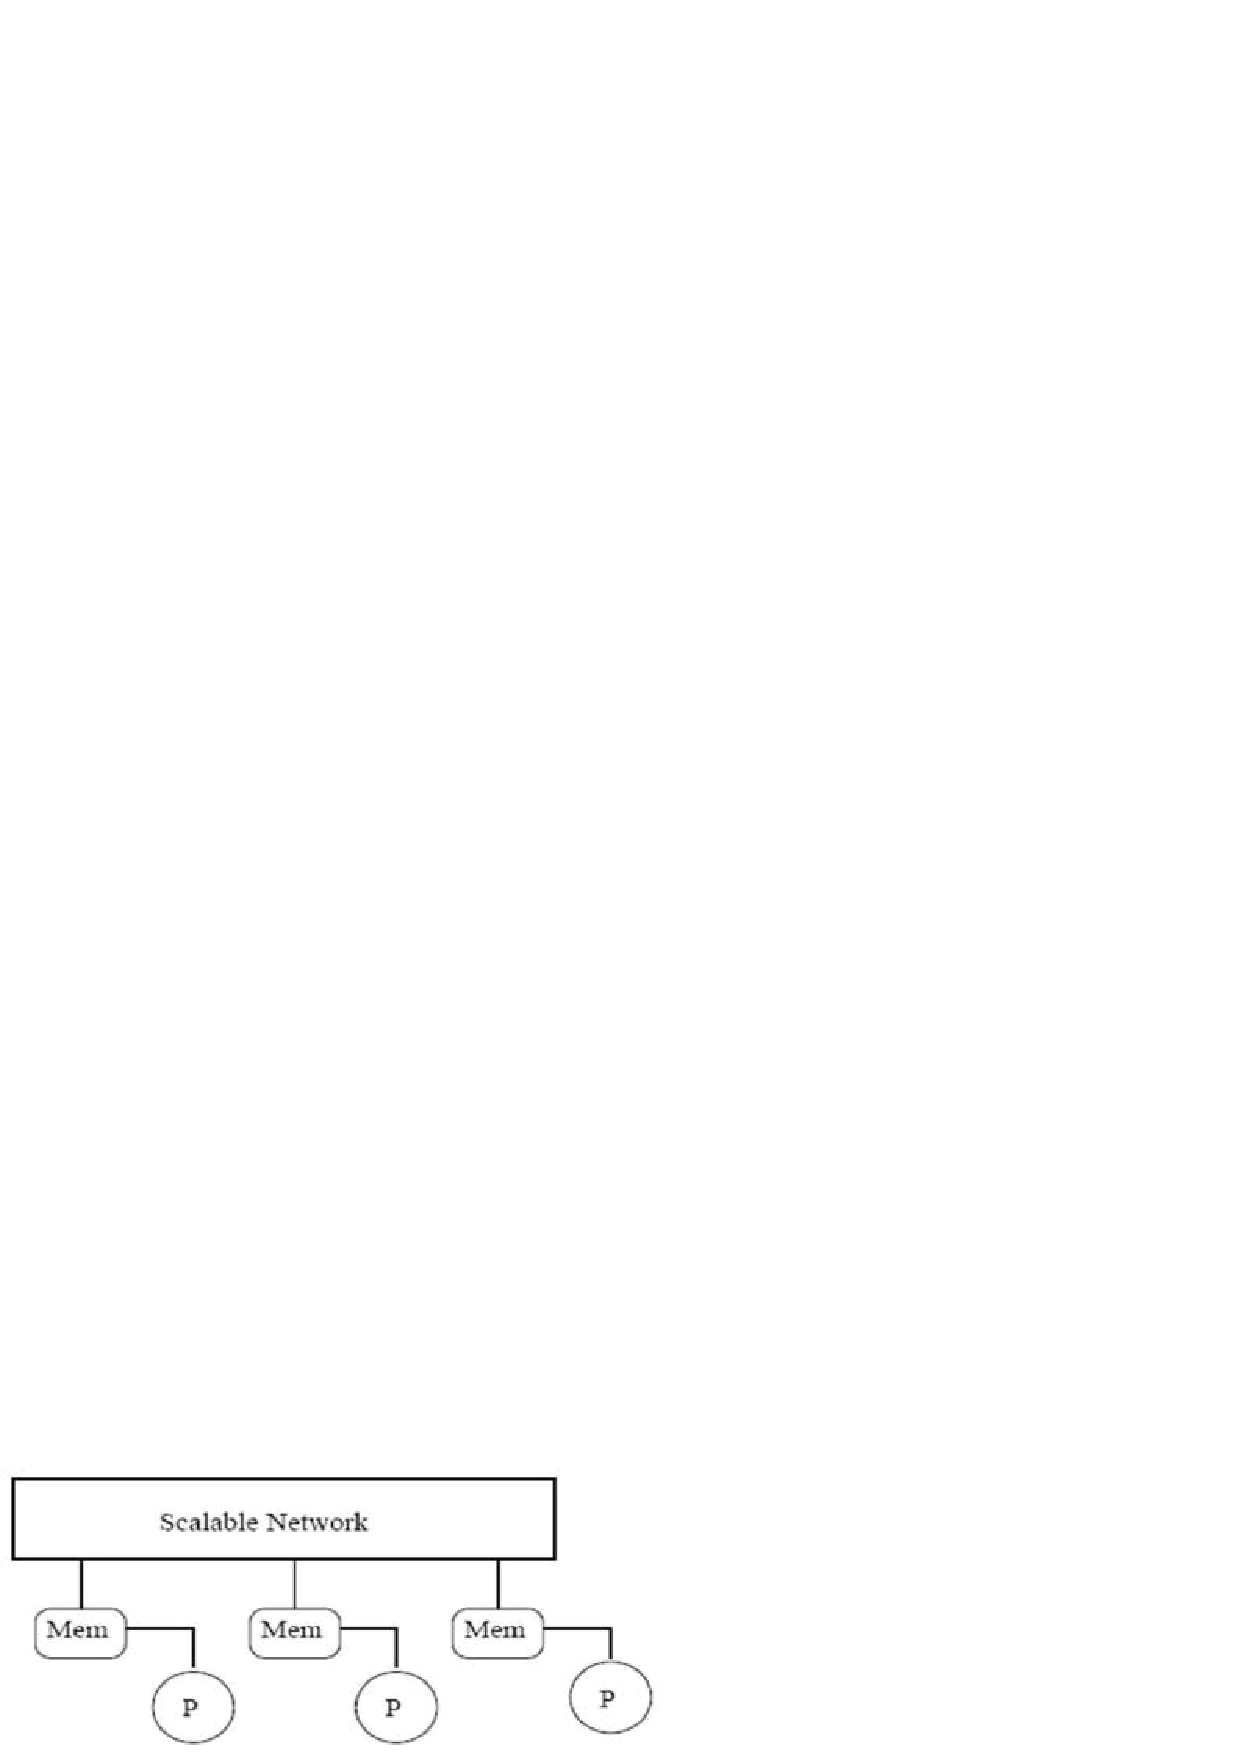
\includegraphics[width=8cm, height=4cm]{./eps/numa.jpg}
 \caption{a simple NUMA architecture design}
 \label{fig:numa}
\end{figurehere}

In Figure \ref{fig:numa} it's possible to see that in a NUMA multiprocessor the physical memory of the system is distributed among individual processors but is still globally addressable by all processors. Sometimes, it is preferable to have more than one processor in the same area. Each of this computational area containing memory block and CPU, whether it has one or more processors, is called node.Thus the cost of a memory access is dependent on where the memory unit addressed is located; relative to the processor some accesses may be local some may be remote. So, with the introduction of NUMA, data locality becomes an important factor because memory accesses have different costs depending on which memory unit is addressed. The scheduling module in the OS must cooperate with the memory management in order to let an application access data mostly from the local memory. NUMA systems can be classified in two categories, both for memory and for processor; regarding memory there are symmetrical and asymmetrical distribution, meaning that accessing different memory nodes can or cannot cost the same. Concerning processor it is possible to have homogeneous system, meaning that all processors are equal in speed and processing power, opposed to heterogeneous ones, where processors have different specifications even inside the same node. This type of architecture turns out to be exposed to some problems, and the most important are: cache coherence, scheduling and memory management and thread migration.\\
In multiprocessor systems it is important to ensure cache coherency. If each processor has a cache that reflects the state of various parts of memory, it is possible that two or more caches may have copies of the same line. It is also possible that a given line may contain more than one lockable data item. If two threads make appropriately serialized changes to those data items, the result could be that both caches end up with different, incorrect versions of the line of memory. In other words, the system's state is no longer coherent because the system contains two different versions of what is supposed to be the content of a specific area of memory. There are 2 types of NUMA architectures that we have to analyse: NCC-NUMA (Non Cache Coherent) and CC-NUMA (Cache Coherent). In NCC-NUMA systems we have some software solutions, while in CC-NUMA we have a cooperation of both software and hardware solutions.\\
Scheduling and memory management are strictly connected; in fact they are used to select the best way to load processes, according to the chosen policy, and decide where to allocate memory concerning that process. The last one is used to decide when it is suitable to migrate a thread from a processor to another one or to a different node; this has an additional cost, due to the migration of the memory associated with the thread. (FIXME....RIVEDERE ULTIMO PARAGRAFO)


%%%%%%%%%%%%%%%%%%%%%%%%%%%%%%%%%%%%%%%%%%%%%%%%%%%%%%%%%%%%%%%%%%%%%%%%%%%%%
\section{Solutions and Methods}

In this chapter will be presented some solutions about the problems introduced in previous section, divided by argument. Evaluations will be considered in the next chapter.

%-----------------------------------------------------------------------------
\subsection{Cache Coherence \\ Section}

As seen before, there are 2 types of NUMA architectures that will be analysed: NCC-NUMA (Non Cache Coherent - NUMA) and CC-NUMA (Cache Coherent - NUMA). \\
In NCC-NUMA systems, [CIT.Shared memory multiprocessing di Norihisa Suzuki ] explain that the inter-cache coherence problem can be solved if shared data, or writable shared data strictly, are not cached with Cacheability Marking Scheme. An attribute bit, called cacheable bit, is provided in each page-table entry to specify whether data in the associated virtual page are cacheable or not. So an OS, with the help of a compiler, marks only virtual pages, which are mapped to either private space or read-only common space, as cacheable pages. When a cache miss occurs on accessing a line of a noncacheable page, an MMU (memory managament unit) does not load the line into the cache. While the page is marked noncacheable, all accesses to the page are always performed in either local or remote memory.\\
Conserning the same problem, [CIT. Software Cache Coherence for Large Scale Multiprocessor - Leonidas I. Kontothanassis and Michael L. Scott] shown a new adaptive algorithm for software cache coherence that reduces interprocessor communication and scales to large numbers of processors; they then evaluate the tradeoffs among various write policies and the effect on performance of using remote memory access. Finally they also observe that certain simple program changes can greatly improve performance.\\
Regarding CC-Numa [CIT. Cache coherency Techniques - Silvia Lametti] explains there are two protocols that are used to guarantee coherence: snooping and directory-based. Snooping system use a totally ordered network to directly broadcast coherence transactions to all processors and memory. Another solution is directory-based protocol; this one transmits coherence transactions over an arbitrary point-to-point network to the corresponding home directories which, in turn, redirect them to the processors caching the line. 

\begin{figurehere}
 \centering
 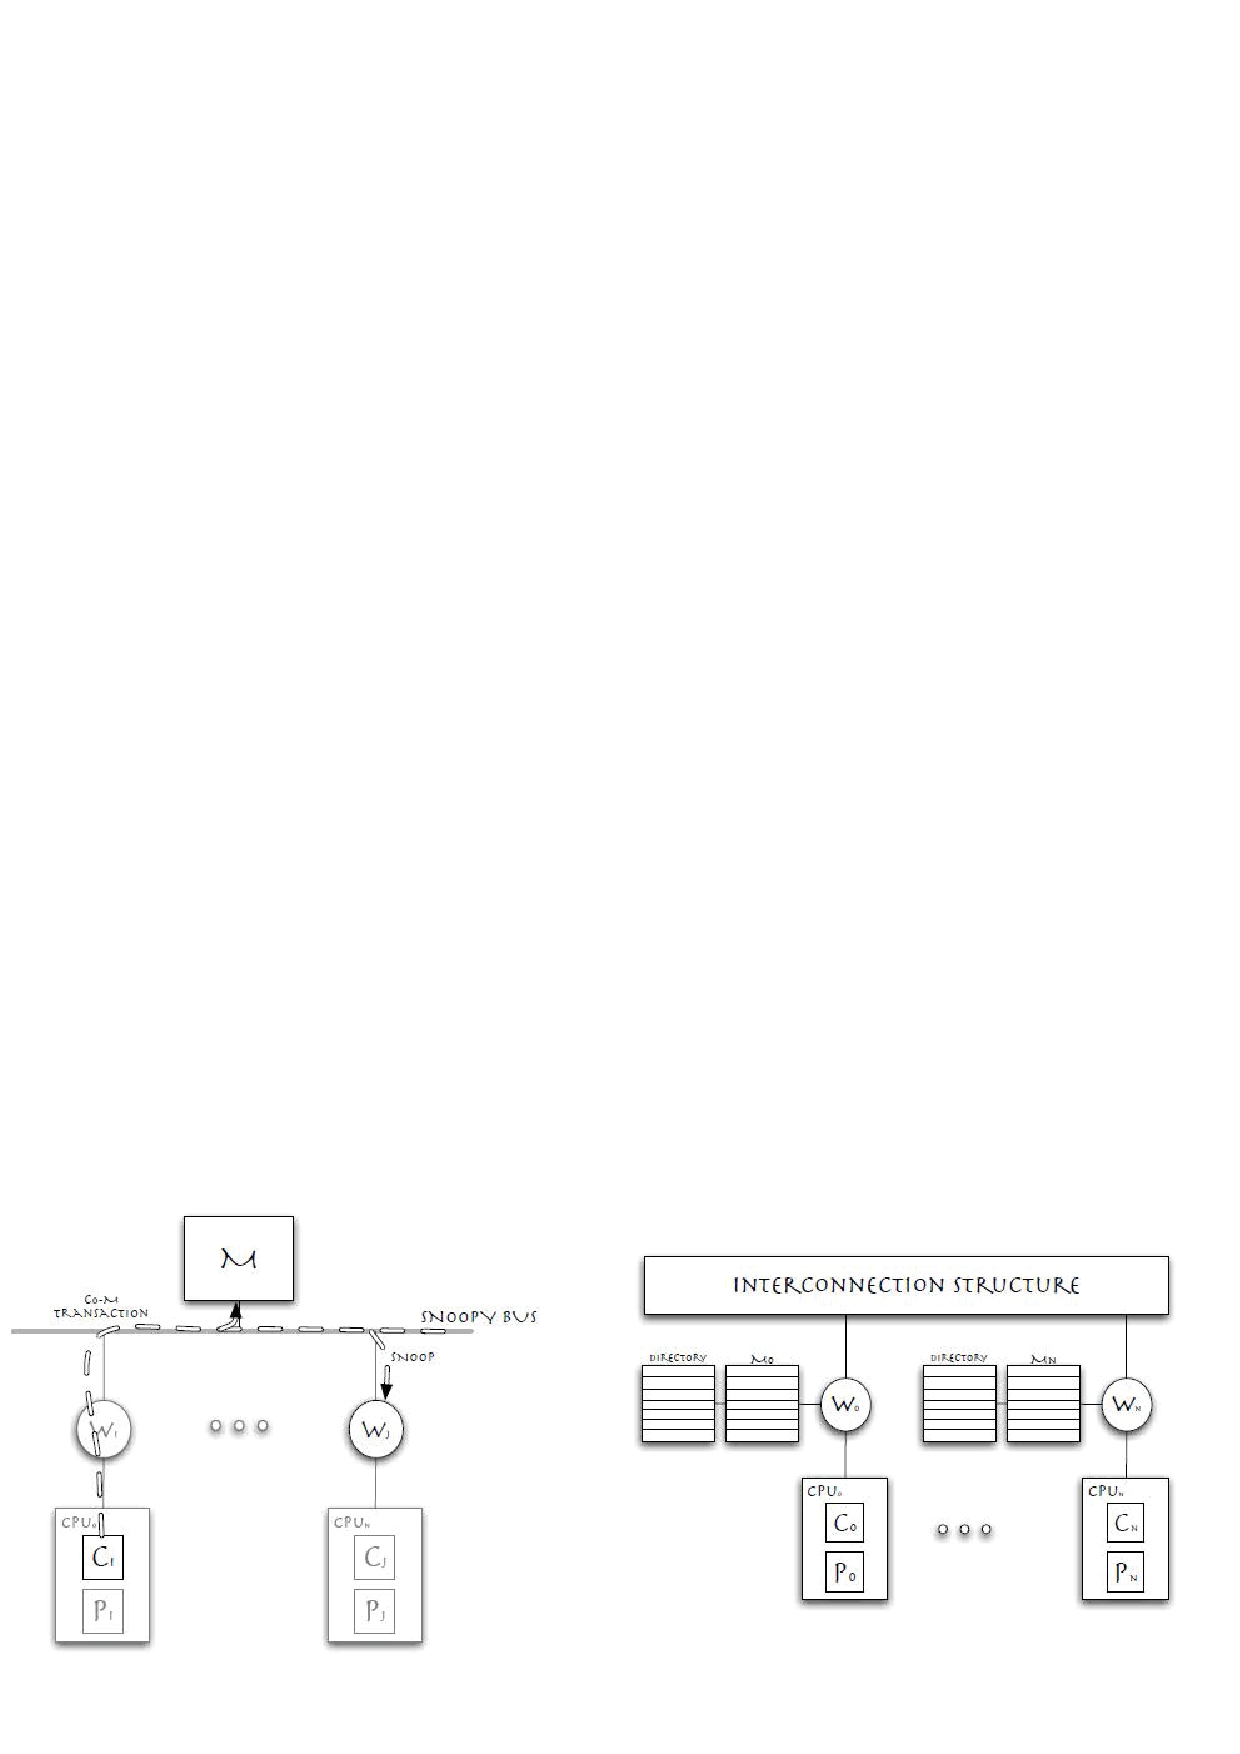
\includegraphics[width=8cm, height=4cm]{./eps/SnoopeDir.png}
 \caption{Snooping and Directory-based protocol}
 \label{fig:s&d}
\end{figurehere}

In all the systems which use the automatic techniques (snooping and directory), a proper protocol must exists in order to perform the required actions atomically. Two main techniques are used: \emph{invalidation}, \emph{update}.\\
Invalidation assumes that the only valid copy of a block is one of those, usually the last one, that has changed, invalidating all other copies (e.g. MSI and MESI in Figure \ref{fig:msimesi}); while update presumes that each modifcation of a cache block copy is communicated (multicasted) to all other caches (e.g. Dragon).

\begin{figurehere}
 \centering
 \includegraphics[width=8cm, height=4cm]{./eps/msimesi.png}
 \caption{MESI and MSI protocol}
 \label{fig:msimesi}
\end{figurehere}

%-----------------------------------------------------------------------------
\subsection{Scheduling and memory management \\ Section}



%%%%%%%%%%%%%%%%%%%%%%%%%%%%%%%%%%%%%%%%%%%%%%%%%%%%%%%%%%%%%%%%%%%%%%%%%%%%%
\section{Evaluation}

In this section it will be discussed the difference between the proposed solutions above giving some value coming from direct confrontation.

%-----------------------------------------------------------------------------
\subsection{Cache coherence \\ Section}


%-----------------------------------------------------------------------------
\subsection{Scheduling and memory management \\ Section}


% We suggest the use of JabRef for editing your bibliography file (Report.bib)
\bibliographystyle{splncs}
\bibliography{Report}

\end{multicols}
\end{document}
